\documentclass{article}
\usepackage{palatino}
\usepackage{graphicx}
\usepackage{listings}
\usepackage{url}
\begin{document}

\lstset{ 
  language=C++,
  belowcaptionskip=1\baselineskip,
  xleftmargin=\parindent,
  basicstyle=\footnotesize\ttfamily
 }

\title{Senior Project: GPU Computing}
\author{John Kloosterman \\
  \texttt{john.kloosterman@gmail.com}}
\date{September 2012-May 2013}
\maketitle


% The final report should be a formal, written paper discussing the nature of the project, the system you built, and the implications for the future. The general sections to include in your final report are as follows:
% Project vision and overview
% Background, including research review
% System design, implementation and testing
% Results and discussion
% Conclusions
% Future work
% Acknowledgements
% References
% Appendixes (if appropriate)
%%%%%%%%%%%%%%%%%%%%%%
\section{Introduction}
This is the introduction.

Main problem I was trying to solve: GPUs are an architecture that has potential for great performance and power improvements, but they are too difficult to use.

Make the parts of your project tell a coherent story about how they fit together. One thing you have done a lot of is algorithms to do fairly simple things on the GPU but don't have a standard library implementation. Idioms like linked lists on CPUs -> idioms like skipping threads for trees on GPUs.

\tableofcontents

%%%%%%%%%%%%%%%%%%%%%%%%
\section{Test Computer}
[introduce test system here]. The system was paid for out of NSF Grant \#XXXX, with the nVidia GPUs provided by nVidia.

\subsection{Hardware}
This system included four different devices that OpenCL supports: an Intel Core i7-3770K CPU, the integrated Intel HD Graphics 4000 GPU, an AMD Radeon 7970 GPU, and two nVidia GTX 480 GPUs.

The theoretical performance of the Radeon 7970 is much higher than all the other devices combined. However, it also had a small maximum workgroup size of 256, whereas the nVidia GPUs supported workgroup sizes of up to 1024.

This system was used for all benchmarks in this report. The CPU used is an Intel Core i7-3770, and the GPU used for benchmarks is the AMD Radeon 7970. The benchmarks were run on 64-bit Ubuntu 12.10.

\subsection{Software Setup}
On Linux, it is currently difficult to have multiple OpenCL platforms installed at the same time. GPU platforms will only work if the X.org driver for that GPU is currently being used, which meant that I could not use the nVidia GPUs when the AMD GPU was being used to drive the display. As well, Ubuntu would not boot with the nVidia graphics drivers installed when the AMD graphics card was installed in the system. On top of this, the nVidia and Intel platforms inmplemented OpenCL 1.1 whereas the AMD platform implemented OpenCL 1.2, and the headers are incompatible between versions even when only OpenCL 1.1 features are being used. For this reason, I developed exclusively with the AMD APP SDK 2.8 on Linux.

The situation is far easier on Windows, where both AMD and nVidia GPUs were always accessible with OpenCL. The Intel integrated GPU was only available if the system was booted with a display connected to it. AMD has the most robust set of tools for profiling and debugging OpenCL, but these tools only work on Windows in Visual Studio. Therefore, my workflow was to develop on Linux, but ensure that the code was portable to Windows, should I need to test on more GPUs and work with the profiling tools available there.

\subsection{OpenCL Quirks}
As of the AMD APP SDK 2.8, for AMD GPUs \texttt{printf()} only reliably works when the tread with local ID (0,0,0) calls it. Sometimes, calls from other threads will make it. As well, \texttt{printf()} often does not work even then if it is inside any kind of conditional structure.

%%%%%%%%%%%%%%%%%%%%%%%
\section{OpenCL Framework}
OpenCL is designed to be flexible, but this means that it is unwieldly for developers to use. The simplest OpenCL program that runs code on a GPU is on the order of 50 lines long. The framework is an attempt at making OpenCL kernel calls syntactially as similar as possible to calling a C++ function or method.

\subsection{Functions vs. Kernels}
The entry point of an OpenCL program is a kernel, marked with the \texttt{\_\_kernel} keyword. This framework wraps around OpenCL's native functionality with the CLKernel class, making it simpler to compile kernels, pass parameters to them, and set the local and global workgroup size of the kernel. An example usage of the CLKernel class is [FILE NAME].

OpenCL does not support calling non-kernel functions, but these functions need some way to be tested. The \texttt{CLFunction} class in this framework removes OpenCL's limitation. A kernel to call the function is automatically generated at compile-time, and that kernel is passed to OpenCL. \texttt{CLFunction} will run the function on one thread.

More complex functions, especially those that involve threads cooperating on a task with data stored in local memory, cannot be called by \texttt{CLFunction}. One idiom I developed when testing these kinds of functions, is to write a shim kernel that copies data into the correct memory space, calls the function to be tested, then copies the results back to \texttt{\_\_global} memory. (See \texttt{societies/util/test/max\_min\_tester.cl.in} for an example)

\subsection{Usage}
C++11 constructs allow a class to syntactically behave like a variadic function, by defining an overloaded () operator using a variadic template. At this time, compilers only partically support the features needed to make using variadic templates elegant. With C++11, a \texttt{CLKernel} or \texttt{CLFunction} can be called like this:

\begin{lstlisting}
#include <CLKernel.h>

string src; // some kernel source code
cl_int i, j, k;
CLKernel theKernel( "kernel_name", src );
theKernel( i, j, k );
\end{lstlisting}

Microsoft Visual Studio 2008 (the version that AMD's OpenCL tools currently target) does not support C++11. This requires a clunkier syntax:

\begin{lstlisting}
#include <CLKernel.h>
#include <vector>

string src; // some kernel source code
cl_int i, j, k;
CLKernel theKernel( "kernel_name", src );

std::vector<CLUnitArgument> arguments;
arguments.push_back( i ); 
arguments.push_back( j ); 
arguments.push_back( k ); 

theKernel( arguments );
\end{lstlisting}

The CLUnitArgument class has constructors for many different types, which means that variables of those types can be passed into a CLKernel or a CLFunction without needing to explicitly create a CLUnitArgument.

\subsection{Other Features}
I found I was often developing on my laptop, which does not have an OpenCL-supported GPU. The framework automatically degrades to using a CPU if there are no GPUs, so that programs will still run, albeit much more slowly in most cases.

If the \texttt{CL\_DEBUG} environment variable is set to 1, the framework will compile kernels with debugging symbols and run them on the CPU. This allows for debugging kernels using gdb as described in the AMD OpenCL programming guide\cite{amdapp}.

\subsection{Memory Copies}
One of the main bottlenecks for GPU computing is the time to transfer data from RAM to the GPU, so the framework needs to avoid making any unnecessary copies. By default, all buffers are copied to and from the GPU every time a kernel is scheduled. This produces correct behaviour at the expense of being slow. The constructor for a \texttt{CLUnitArgument} allows developers to specify whether the host memory backing the buffer should be copied to or from the GPU.

\subsection{Lazy Initialization of Buffers}
In order that \texttt{CLUnitArgument}s can be instantiated implicitly by the C++ compiler, their constructors may not take an OpenCL context object. This object is needed in order to create the \texttt{cl::Buffer} that the \texttt{CLUnitArgument} encapsulates. It is passed later to the object by a \texttt{CLFunction} or \texttt{CLKernel} when the \texttt{cl::Buffer} is needed for the first time.

This causes undesired behaviour if a copy of an original \texttt{CLUnitArgument} is what initializes the \texttt{cl:Buffer}, because the reference to the \texttt{cl::Buffer} does not propagate back to the original. C++ creates copies of \texttt{CLUnitArgument}s implicitly whenever they are used as arguments to \texttt{CLKernel}s or \texttt{CLFunction}s. Besides there being extraneous buffers created, this makes it impossible for \texttt{CLUnitArgument}s to store data on the device without copying it back to the host. Code like this then breaks:

\begin{lstlisting}
cl_float array[1024];
CLUnitArgument arrayArg( "float", array, 1024, false, false );
someKernel( arrayArg ); // stores data into arrayArg, doesn't copy
                        // data back to host.
someOtherKernel( arrayArg ); // reads data someKernel() stored.
\end{lstlisting}

The \texttt{CLUnitArgument::makePersistent()} method solves this problem by giving developers a way to create the \texttt{cl::Buffer} before any copies of the \texttt{CLUnitArgument} are made. For an example of where this is necessary, see \texttt{OpenCLPlayer::makeMove()} in \texttt{kalah/opencl\_player.cpp}.

\subsection{Examples}
There is an example usage of this framework in the \texttt{cl\_test/example} directory. All the other components of my project used this library as well, which means they serve as more complicated usage examples.

%%%%%%%%%%%%%%%%%%%%%%
\section{Raytracer}
As a simple application to run on top of my framework, I implemented an OpenCL raytracer for honours credit in CS 352 (Computer Graphics). The raytracer maps one pixel onto one hardware thread. The objective was for the raytracer to support real-time user interaction.

\subsection{Capabilities}
The raytracer has two geometric primitives: spheres and planes. Geometry can have a solid colour or be reflective. There can be any number of geometric primitives.

The lighting model takes into account ambient and diffuse lighting. There can be any number of diffuse light sources.

\subsection{Limitations}
Because OpenCL does not support recursion, reflective surfaces do not behave as they do in other raytracers. Reflective surfaces shoot a ray off the reflective surface, and the ray takes the colour of the first object it hits, taking into account only ambient lighting (see Figure \ref{fig:reflections}). Other raytracers are able to take into account other types of lighting from the reflected surface, and can simulate rays being reflected more than once. This is not possible with this implementation, because it would involve a recursive call from the lighting function to the lighting function.

\begin{figure}[ht!]
\centering
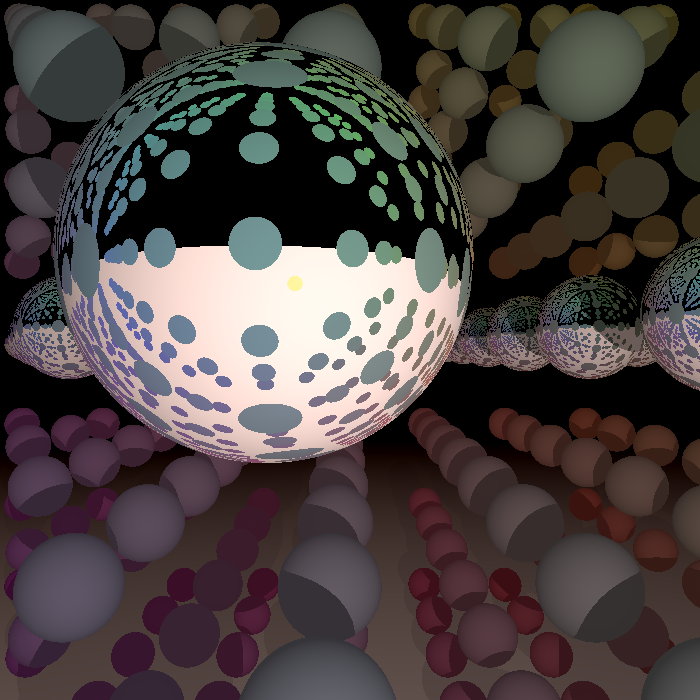
\includegraphics[width=90mm]{reflections.png}
\caption{Reflections that only take into account ambient lighting}
\label{fig:reflections}
\end{figure}

\subsection{User Interface}
The user interface was implemented in GTK+, with the rendered image being displayed in a \texttt{GtkImage}. This is inefficient, as the image is rendered on the GPU, copied to the CPU, copied to the \texttt{GtkImage}, then pushed back to the GPU. An alternative that trades increased complexity for more performance would be taking advantage of OpenCL's OpenGL interoperability features to draw the image.

\subsection{Performance}
The raytracer is able to render a 700x700 pixel test scene with 1000 spheres and a moveable diffuse light source at speeds that make it interactive (see figure \ref{fig:testscene}). Using the CPU, this scene takes 1.28 seconds per frame (0.78 frames per second). Using the Radeon 7970, the scene takes 0.055 seconds per frame (18 frames per second). If the number of spheres is reduced to 216, the Radeon 7970 can render the scene at 60 frames per second.

\begin{figure}[ht!]
\centering
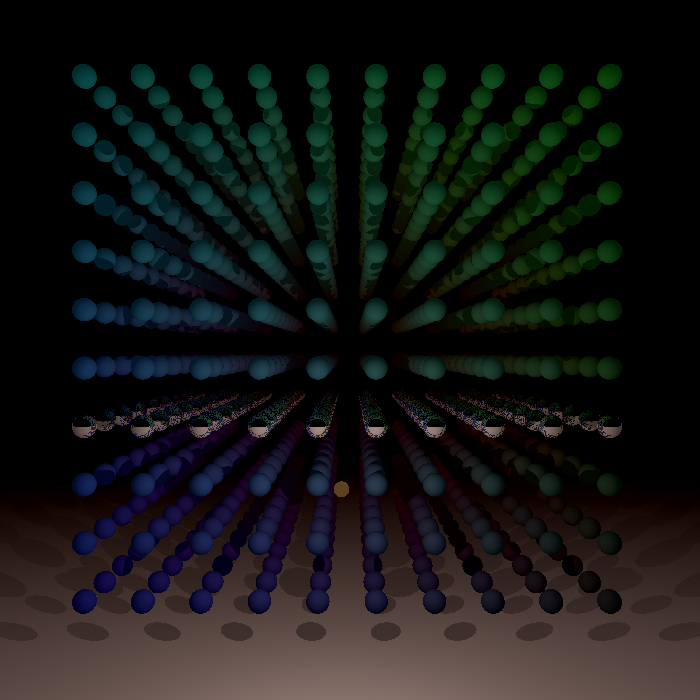
\includegraphics[width=90mm]{scene.png}
\caption{Test scene, featuring 1000 spheres and ground plane}
\label{fig:testscene}
\end{figure}

\subsection{Discarding Frames}
The sliders generate GTK+ events, which are processed in callback functions like \texttt{motion\_notify()}. These callbacks call \texttt{run\_kernel()}, which renders the frame. This blocks the main program thread, but mouse drag events on the image still get queued. The effect is that the program can get more and more behind when rendering frames if events are added faster than frames can be rendered. This makes the raytracer feel unresponsive.

To prevent this from happening, after rendering a frame, the callbacks discard all the events on the GTK+ event queue that could cause a new frame to be rendered. This is done by having an \texttt{in\_handler} flag that is set when a callback that is rendering a frame is running. All callbacks that can render a frame check to see if \texttt{in\_handler} is set, and if so, return without rendering the frame. Immediately after rendering a frame, a callback runs this loop:

\begin{lstlisting}
while ( gtk_events_pending() )
  gtk_main_iteration();
\end{lstlisting}

This causes all the queued GTK+ events to be processed; because the \texttt{in\_handler} flag is set, any other callbacks in the queue do not render a frame. The end result is that all the events that could render a new frame are flushed from the queue.

%%%%%%%%%%%%%%%%%%%%%%%%%%%%%%%%%5
\section{Mankalah Minimax AI}
This part of the project implemented a minimax player for the Mankalah game introduced in CS 212. Minimax is a much harder algorithm to implement on a GPU than a raytracer, because the minimax tree has dependencies between nodes, and the parallelism is less obvious.

\subsection{Strategy}
Following previous work on another minimax player implemented in CUDA\cite{rockisuda10}, the minimax tree is broken up into layers. On the CPU, the first layers of game boards in the minimax tree are computed and the bottom-level leaf nodes of that tree are put into a C++ vector. The boards in the vector are copied over to the GPU, where 4 more levels of minimax are computed. Because the Mankalah minimax tree has a branching factor of 6, the overwhelming majority of the work is done in the bottom 4 levels of the tree (see figure \ref{fig:minimaxdiagram}).

\begin{figure}[ht!]
\centering
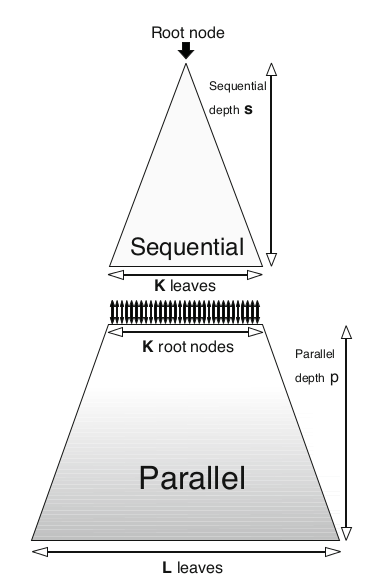
\includegraphics[width=50mm]{minimax-diagram.png}
\caption{Sequential and parallel segements of minimax tree, taken from Rocki and Suda\cite{rockisuda10}.}
\label{fig:minimaxdiagram}
\end{figure}

The algorithm run on the GPU for evaluating the bottom layers of the minimax tree is as follows:

\subsubsection{Generating boards}
In this step, the game boards that represent the game tree for the next number of moves are generated from the start board. The tree is stored in global memory in an array, where the child of the node stored at location n in the array is at location 6n + 1. This can be computed in O(log(n)) time with $n^{d}$ threads, by having the first thread compute the first node, 6 threads compute the first level of child nodes, 36 threads compute the second level, and so on.

\subsubsection{Evaluating boards}
In the standard minimax algorithm, the evaluate function needs to be computed only for boards at the leaf nodes of the game tree. Because all threads execute the same instruction counter, however, it is not slower to run the function on all the generated boards. This saves time in a later step, as should the game end at a stage before the bottom level of the minimax tree, the board is already evaluated.

\subsubsection{Minimax}
The minimax scores at a node can be computed in O(log(n),n) time by using $n^{d-1}$ threads to compute the minimax values for the nodes one level above the leaf nodes, $n^{d-2}$ threads to compute the minimax values for the nodes 2 levels about the leaf nodes, and so on. After this process, the parent node for the game tree stores the minimax value for the tree.

\subsubsection{Limitations}
Because the boards are stored in local memory, and there are sequential dependencies between these steps, all threads for one of these minimax trees must be in the same workgroup. On the Radeon 7970, the maximum work group size is 256. Therefore, for Kalah, with a branching factor of 6, a minimax tree of 4 levels ($6^0 + 6^1 + 6^2 + 6^3 = 259$ nodes) was used, with a workgroup size of $6^3 = 216$. Since there were more nodes in the tree than threads in the workgroup, some threads had to evaluate 2 boards.

\subsection{Increasing Search Depth}
Because of memory bottlenecks, there is a limit to how many GPU minimax instances can be dispatched efficiently. On the test system, 8 levels of sequential minimax (genering an average of [--] GPU instances) was optimal for performance. As well, as Rocki and Suda\cite{rockisuda10} noted, the search tree has to be traversed twice at this level, once to determine what the leaf nodes are, and second to run the minimax reduction on the nodes.

Therefore, to gain more search depth, another level of sequential minimax was run above this first round of sequential minimax. Adding more levels at the topmost level of minimax increased the depth of the search but not the number of GPU instances dispatched at one time. Only one traversal of the search tree is necessary at this step.

\subsection{Performance}
\subsubsection{Optimal Sequential Depth}
One optimization question is for a minimax tree of a given depth how many levels shuld be computed in each of the 3 minimax stages. The GPU portion is fixed at 4 levels, so the distribution needs to be between the two sequential minimax stages. On the test system, the optimal allocation was XXXXXXXXXXX.

REDO THIS, because for depth 13, (0,10) is fastest, but (0,11) is too large for the GPU. It would make more sense to do depth 14, even though ti would take longer to benchmark.

\begin{tabular}{| l | l | l | l | l |}
  \hline
  Pre & Seq & Parallel & Time for 20 & Time for 1 \\
  \hline
  0 & 10 & 4 & 188.03s & 9.40s \\
  1 & 9 & 4 & 221.17s & 11.05s \\ 
  2 & 8 & 4 & 212.45s & 10.62s \\
  3 & 7 & 4 & 233.92s & 11.70s \\ 
  4 & 6 & 4 & 281.78s & 14.09s \\
  \hline
\end{tabular}

\subsubsection{Speedup}
A recursive sequential algorithm was implemented for performance comparisons. As the table below demonstrates, the using the GPU yielded about a 10x speedup once the problem became sufficiently large. A 10x performance increase for a game with a branching factor of 6 means that the player can look another move ahead in the game.

\begin{tabular}{| l | l | l | l | l |}
  \hline
  Depth & Sequential (s) & CPU OpenCL (s) & GPU OpenCL (s) & Speedup\\
  \hline
  4 & 0.000068 & 0.000656 & 0.000919 & 0.07x \\
  5 & 0.000343 & 0.008957 & 0.000907 & 0.37x \\
  6 & 0.001658 & 0.004544 & 0.001054 & 1.57x \\
  7 & 0.008301 & 0.023702 & 0.001382 & 6.00x \\
  8 & 0.040561 & 0.102351 & 0.005487 & 7.39x \\
  9 & 0.203477 & 0.516266 & 0.021644 & 9.40x \\
  10 & 0.980497 & 2.61265 & 0.1048 & 9.35x \\
  11 & 4.80143 & 11.0873 & 0.438745 & 10.9x \\
  12 & 23.4349 & 60.0211 & 2.23596 & 10.5x \\
  13 & 113.512 & 231.792 & 9.41622 & 12.1x \\
  \hline
\end{tabular}
Since minimax is an embarrasingly parallel problem, a parallel CPU implementation should be able to achieve a speed of $\frac{sequential}{\# cores}$. Since the OpenCL parallel implementation was worse on the CPU than the sequential implementation, which itself can be sped up 4 times on the test system, this illustrates how algorithms tuned for GPUs are very different than ones tuned for CPUs.

\subsection{Testing}
Along with testing of each of the GPU minimax algorithm's components, I used fuzz testing to ensure that the output of the GPU minimax algorithm was the same as the output of the sequential CPU minimax implementation. This was done by generating random valid boards then running both algorithms on them and comparing the output.

\subsection{Sharing Code Between Host and Device}
In order to avoid code duplication for the logic for Mankalah boards, the code in \texttt{board.c} and a few other files is used both on the host and device side. To consolidate all a kernel's dependencies into one file, I used the preprocessor to \texttt{\#include} many \texttt{.c} files into one source file. I have tried consistently use the extension \texttt{.cl.in} for OpenCL source files that need to be preprocessed before they will compile.

For data structures passed between the host and device, a shared header file can be used. However, it is important to ensure that the layout of the structures are exactly the same. Notably, fundamental times like an \texttt{int} on the device side is not guaranteed to be the same size as an \texttt{int} on the host side. OpenCL provides types on the host prefaced with \texttt{cl\_} that are guaranteed to be the same size as the type without the prefix on the client side (for an \texttt{int} on the device side, a \texttt{cl\_int} is necessary on the host side). I used preprocessor macros to use the correct types depending on where code is compiled.

\subsection{Tree Structures in OpenCL}
Because there is no dynamic memory allocation in OpenCL, I have stored all trees in arrays. It is common to store binary trees in arrays, where the first child of the node at location $n$ is at location $2n$, and the second at $2n + 1$. This can be generalized to trees of other branching factors. A few support functions for this data structure can be found in \texttt{kalah/tree\_array.c}.

%%%%%%%%%%%%%%%%%%%%%%%%%
\section{Economics Simulation}
As a larger, more complex problem, I worked on implementing a GPU version of an economics simulation used for research in Calvin's economics department.\cite{ditta13} The simulation already exists in Python, but it takes on the order of weeks to run. The simulation consists of a number of agents, which each hold a number of resources, that can harvest resources, invent machines to make harvesting resources more efficent, and trade resources and machines with each other.

This problem has promise for a speedup with a GPU's massive parallelism. Each of the agents in the simulation is largely independent, and most of the decisions that agents have to make need to evaluate the relative worth of their resources. Therefore, there is a natural mapping of one hardware thread to one resource, with each agent mapped to its own workgroup.

I did not complete the reimplementation of the simulation, but have met my objective of applying GPU computing to a complex, real-world problem. The Societies paper\cite{ditta13} breaks the simulation into 6 phases, of which the first 3 are non-trivial, the fourth is very complex, and the last 2 are trivial. I implemented the first 2 phases. This was enough to encounter difficult problems that required very different algorithms to efficiently solve on a GPU.

\subsection{Phase 1: Resource Extraction}
In this phase, agents harvest resources while there is time left in the ``day''. In each round, agents choose one of the resources that is most valuable for them to have one more unit of. Agents gain experience extracting resources, which reduces the amount of time needed to extract that resource.

The challenges implementing this phase were implementing the maximum and minimum algorithms, creating a mechanism for threads to create a variable-size array of options, and finding a random number generator.

\subsubsection{Array Maximum and Minimum}
Several times in this simulation, I needed to find the maximum or minimum in an array without modifying the values in the array. The most efficient way to do this with at least 1 thread for every 2 elements is to build a max/min tree, since this allows the maximum or minimum to be found in O(log(n),n) time. Unfortunately, for an array with n elements, this requires a scratch array in \texttt{\_\_local} memory of $\frac{n}{2}$ elements.

The algorithm has two phases. In the first phase, $\frac{n}{2}$ threads compare 2 elements of the original array, and put the largest in the scratch array. In the second phase, $\frac{n}{4}$ threads compare 2 elements of the scratch array, and put the maximum/minimum of the two values in the location of the first value. The second phase iterates, each time with half as many threads, until there is one value left, which is the minimum/maximum.

The implementation of this algorithm is in \texttt{societies/util/max\_min.cl}. This implementation also includes the ability to pass in a mask array, which allows the algorithm to ignore certain values in the array. This permits using the algorithm multiple times to find the maximum/minimum n elements in an array. (See the \texttt{max\_n\_indices()} function.)

\subsubsection{Variable-length Arrays}
There are cases where one thread needs to make a choice between different values on behalf of the workgroup. One implementation of this idiom can be found in \texttt{societies/util/choose\_thread.cl}, where several threads can register their ability to be chosen, then one thread randomly makes a choice between them. Since not all threads want to be chosen, there needs to be a data structure that can hold a variable number of elements and that all threads can add elements too.

This data structure can be implemented in OpenCL with an atomic counter variable in \texttt{\_\_local} memory initialized to 0, with an array in \texttt{\_\_local} memory that is large enough for the maximum possible number of elements. When a thread wants to add an element, it calls the OpenCL-builtin \texttt{atomic\_inc()} function to increment the counter, and puts a value in the array at the position that \texttt{atomic\_inc()} returns, which is the previous value of the counter variable. After all threads have finished adding values to the array, the counter variable holds the number of items in the array.

\subsubsection{Random Numbers}
Many of the Societies algorithms required a source of random numbers. On a GPU, this is difficult because there is no hardware source of random numbers, and PRNGs require a unique seed per workgroup so that each workgroup does not generate the same sequence of random numbers. I made use of the MWC64X random number generator, which is ideal for GPUs because it requires very little state to be preserved across runs. I found an OpenCL implementation which was verified against statistical tests.\cite{mwc64x}

\subsection{Phase 2: Resource Trading}


\subsection{Testing}
One weakness of the Python Societies code is that it is not written in a way that makes it easy to test. I made sure to make my code very clean  and wrote unit tests for all my functions, so that my code will be useful to the Societies project in the future. The algorithms I developed to find the maximum and minimum elements in an array I was also careful to test; this code should be useful as a reference for others doing similar work in OpenCL.

\subsection{Kernel Size}
The OpenCL kernels for Societies were relatively large. This is because \texttt{\_\_local} memory cannot be preserved across kernel runs, so splitting up complex tasks into several kernels was not feasible. The Mankalah player has 3 stages that are independent except that the values in \texttt{\_\_local} memory needed to be kept. This is a limitation of the hardware that leaks through as complexity for programmers.

My strategy was to test each of the segments of the kernels independently, so that it was still possible to debug one section of code at a time. However, certain kinds of bugs like race conditions due to missing barriers can only be tested with the kernel as a whole.\footnote{As an aside, CPUs are much more vulnerable to synchronization errors than GPUs, because on a GPU, all hardware threads in a workgroup share an instruction pointer. In fact, the AMD OpenCL backend removes barriers that are made unnecessary by the GPU's architecture.}

\subsection{Configuration Values}
There were several configuration values that are known at kernel compile time, but at host run time. Some of them, like the number of agents in the simulation, needed to be accessible as preprocessor macros. Another advantage of passing configuration values from the host to the device using preprocessor macros rather than inside a configuration object is that memory accesses can be cut out of 

\section{\_\_local Memory malloc()}
One problem I ran across when implementing the Societies code was that most functions required many parameters to pass around scratch \texttt{\_\_local} memory that was needed by some algorithm several function calls deep. These scratch buffers needed to be declared at the beginning of a kernel rather then when they were actually used, and I had to keep track of exactly how large they needed to be. Also, because \texttt{\_\_local} memory usage restricts the number of hardware threads that can be concurrently running on the GPU, it is important to minimize the amount used, which means reusing the same buffers when possible. The result is that the complexity of managing buffers of \texttt{\_\_local} memory became a bottleneck.

Because the sizes of all these buffers is known at compile-time, and OpenCL does not support recursion or function pointers, simple static analysis is enough to determine the maximum amount of \texttt{\_\_local} memory a kernel needs. This should make it easy to shift the accounting burden from the programmer onto a tool.

As well, OpenCL does not support global variables, so any state used by a \texttt{malloc()}-like tool needs to be passed as a parameter to every function. This is inconvenient for the programmer, and should be easy for a tool to write into a program.

\subsection{Integration with Clang}
The Clang C-family compiler is written to be extensible. Clang's abstract syntax tree (AST) includes references to the text that every AST node is built from, which is meant to make it easy for tools to analyze and rewrite source code. Clang's \texttt{Rewriter} class allows for sections of source code to be added, deleted, and moved around. Clang also is used in many OpenCL vendors' backends, which means it natively supports the OpenCL keywords like \texttt{\_\_kernel} and adds these annotations to its AST.

Therefore, this tool links against Clang, and creates an instance of an OpenCL compiler that does semantic analysis but stops before code generation. By using Clang's AST nodes and its \texttt{Rewriter} class, this tool offloads the heavy lifting of parsing and rewriting C source code to Clang.

Because of the tight integration with Clang, the tool is vulnerable to modifications to Clang's internals. The tool was developed against Clang 3.2 and LLVM 3.2.

\subsection{Phase 1: Computing Maximum Allocation}
The tool registers hooks into Clang's AST processing methods. Whenever a function declaration is encountered, the tool generates a new node in a call graph. Then, whenever a function call or a call to \texttt{local\_malloc()} or \texttt{local\_free()} is encountered, the tool adds these actions to the node in the call graph. Clang's AST nodes for the \texttt{local\_malloc()} and \texttt{local\_free()} have methods that make it easy to get a numerical value for the amount of memory allocated or freed, even when that value is an expression or defined by a preprocessor macro.

After all nodes in the AST have been visited, this call graph is guaranteed to have no cycles, because OpenCL does not support recursion. Therefore, in this call tree, the maximum amount of memory allocated by a function is the maximum amount allocated by any of a function's children plus any memory the function has allocated at the same time.

\subsection{Phase 2: Program Rewriting}
The tool then revisits all the nodes in the AST again, and rewrites function declarations and calls. To the kernel function, it inserts initialization code and allocates the \texttt{\_\_local} memory buffer at the size computed in the previous phase. The tool adds a state object to every function call and declaration, so that that state object is accessible anywhere in the program.

\subsection{Including Runtime Code}
The actual code for the \texttt{local\_malloc()} and \texttt{local\_free()} functions needs to be bundled with the rewritten code. One difficulty is that these functions have a different signature before and after rewriting (because the state object is added as a parameter). Also, OpenCL does not support including header files in its compiler. Therefore, the rewriter injects the needed run-time code at the beginning of the program, with the signatures of \texttt{local\_malloc()} and \texttt{local\_free()} as the programmer expects them defined as prototypes. These prototypes are visible only when a preprocessor macro is defined. This allows Clang to parse the code without errors. This code is left in after rewriting, but the preprocessor macro is no longer defined. This exposes the run-time signatures of \texttt{local\_malloc()} and \texttt{local\_free()} along with their code.

I wrote a small tool that allowed me to embed this source code into the executable of the tool, which means that the tool does not need to find that source code to be able to run.

\subsection{Results}
An example program using \texttt{local\_malloc()} is in \texttt{local\_malloc/example}.

%%%%%%%%%%%%%%%%%%%%%%%%%%%%%%%%%%%%%%%%%5
\section{Conclusions}

%%%%%%%%%%%%%%%%%%%%%%%%%%%%%%%%%%%%%%%%%%%
\section{Future Work}


\bibliographystyle{plain}
\bibliography{final-report}

\end{document}
